\documentclass[../main.tex]{subfiles}
\graphicspath{{\subfix{../Figures/}}}

\begin{document}

\chapter{Supplementary visualizations}
\label{ch:plots}

\begin{figure}
    \centering

    \begin{subfigure}[b]{\textwidth}
        \centering
        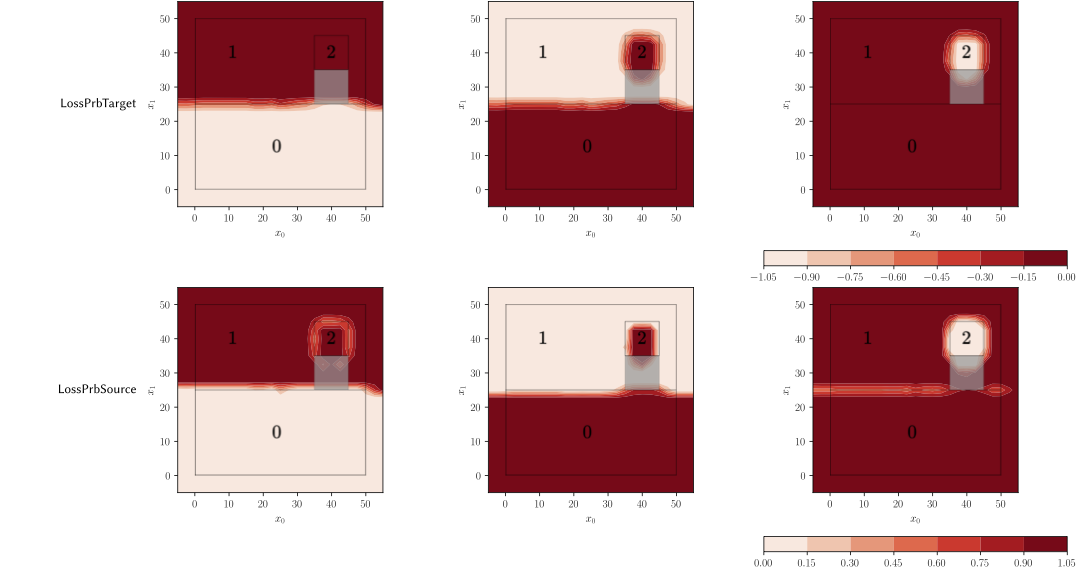
\includegraphics[width=\textwidth]{./05_cf_losses/Appendix/x_losses_prb.png}
        \caption{Probability-based losses with $\lambda=1$.}
    \end{subfigure}
    \begin{subfigure}[b]{\textwidth}
        \centering
        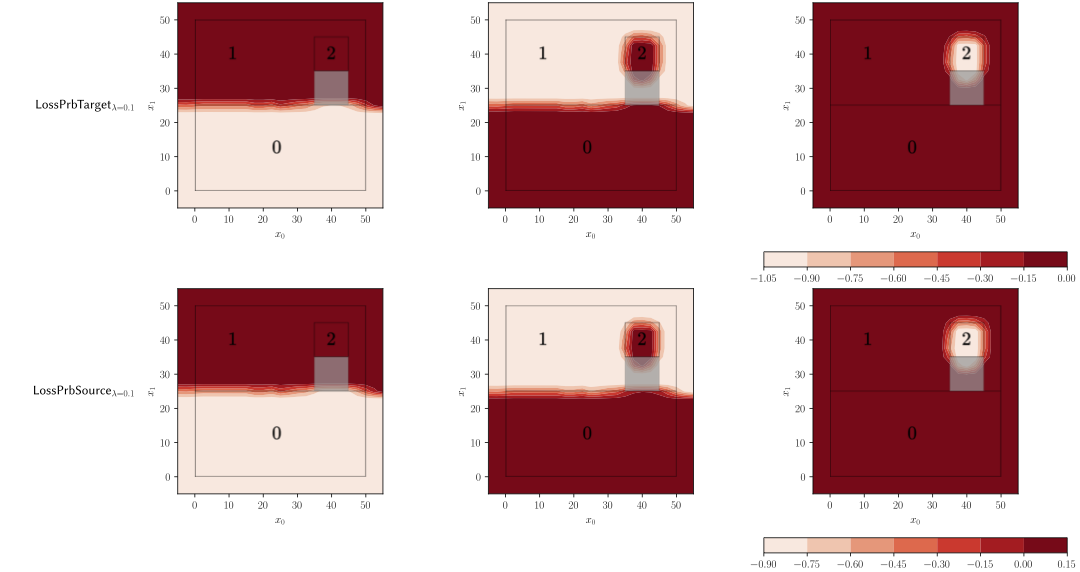
\includegraphics[width=\textwidth]{./05_cf_losses/Appendix/x_losses_prb01.png}
        \caption{Probability-based losses with $\lambda=0.1$.}
    \end{subfigure}
\end{figure}
\begin{figure}\ContinuedFloat
    \centering
    \begin{subfigure}[b]{\textwidth}
        \centering
        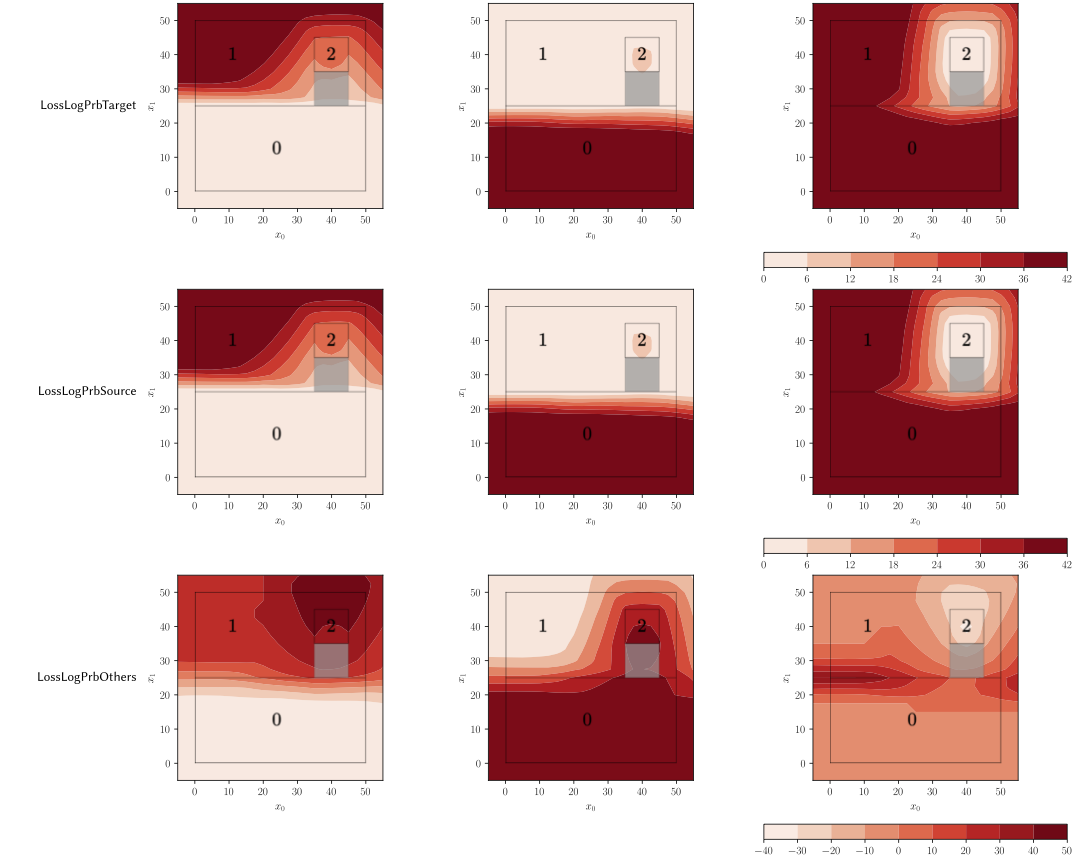
\includegraphics[width=\textwidth]{./05_cf_losses/Appendix/x_losses_logprb.png}
        \caption{Log-probability-based losses with $\lambda=1$.}
    \end{subfigure}
    \begin{subfigure}[b]{\textwidth}
        \centering
        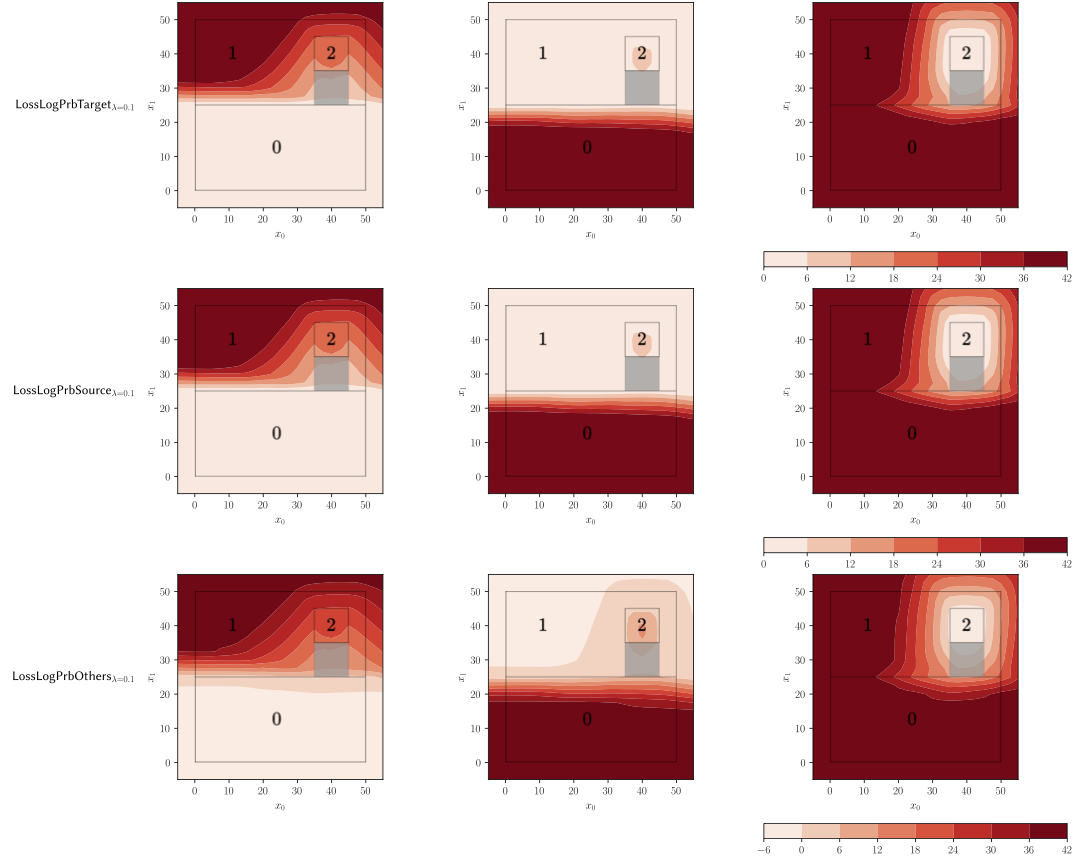
\includegraphics[width=\textwidth]{./05_cf_losses/Appendix/x_losses_logprb01.png}
        \caption{Log-probability-based losses with $\lambda=0.1$.}
    \end{subfigure}
\end{figure}
\begin{figure}\ContinuedFloat
    \begin{subfigure}[b]{\textwidth}
        \centering
        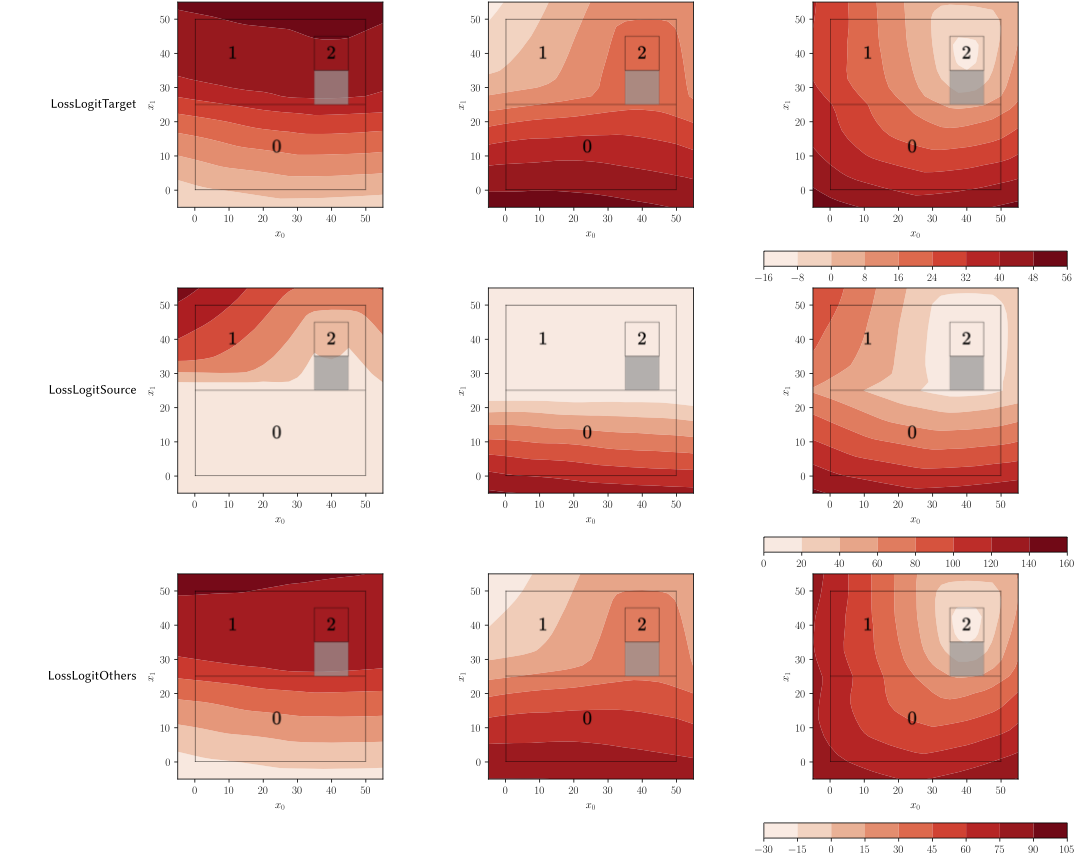
\includegraphics[width=\textwidth]{./05_cf_losses/Appendix/x_losses_logit.png}
        \caption{Logit-based losses with $\lambda=1$.}
    \end{subfigure}
    \begin{subfigure}[b]{\textwidth}
        \centering
        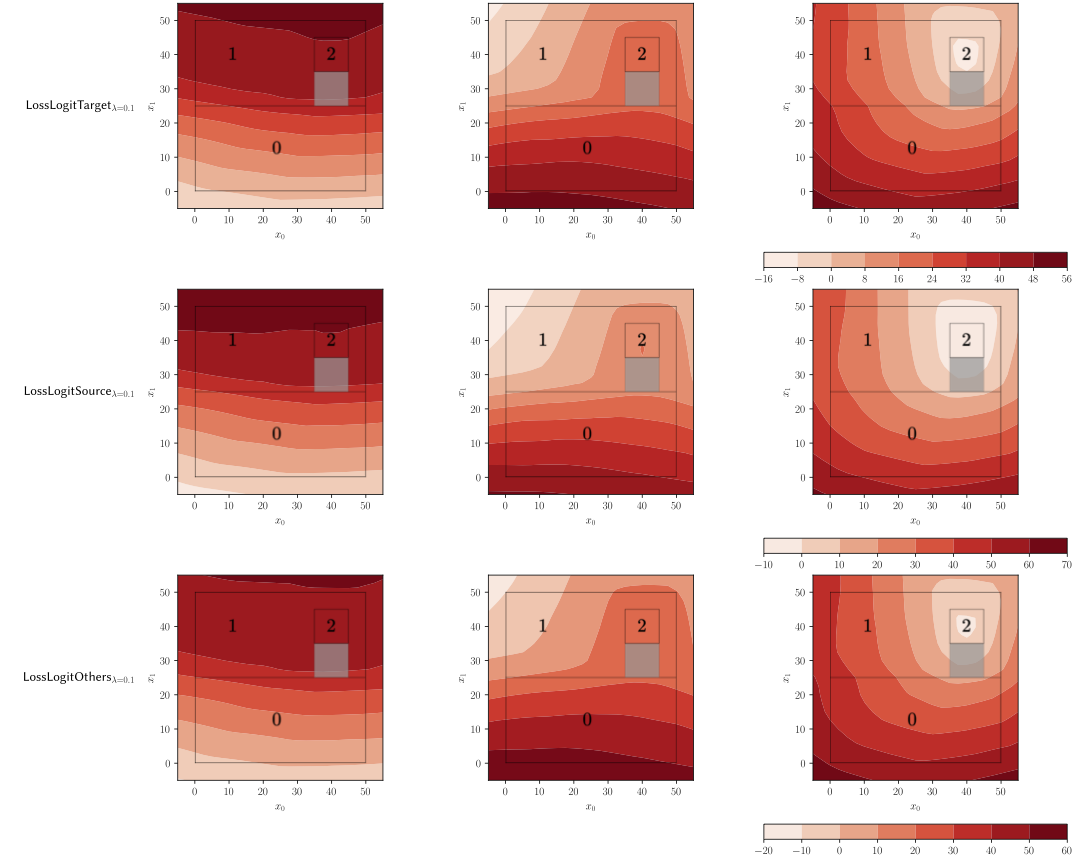
\includegraphics[width=\textwidth]{./05_cf_losses/Appendix/x_losses_logit01.png}
        \caption{Logit-based losses with $\lambda=0.1$.}
    \end{subfigure}

    \caption{Validity losses on \CakeOnSea. The column indicates the target class (0 on the left, 1 in the middle, 2 on the right). Each colorbar applies to the row of plots right above it.}
\end{figure}

\begin{figure}
    \centering

    \begin{subfigure}[b]{\textwidth}
        \centering
        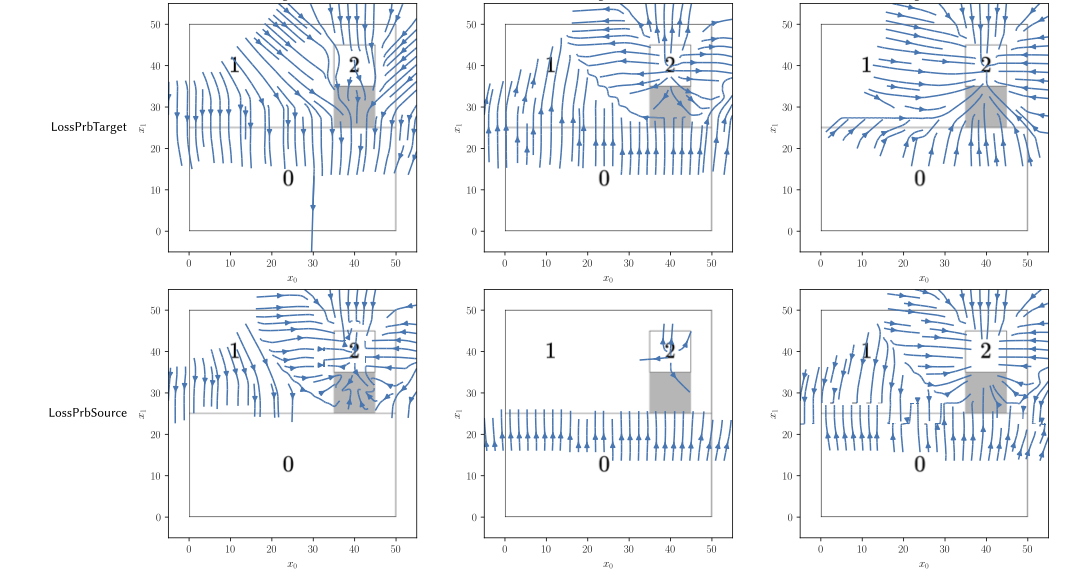
\includegraphics[width=\textwidth]{./05_cf_losses/Appendix/x_gradients_prb.png}
        \caption{Probability-based losses with $\lambda=1$.}
    \end{subfigure}
    \begin{subfigure}[b]{\textwidth}
        \centering
        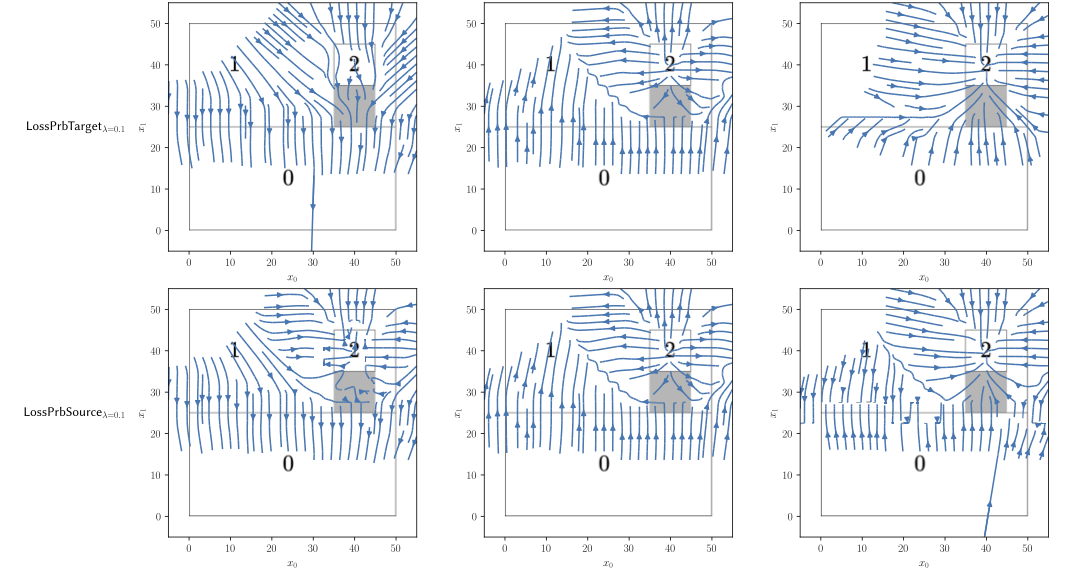
\includegraphics[width=\textwidth]{./05_cf_losses/Appendix/x_gradients_prb01.png}
        \caption{Probability-based losses with $\lambda=0.1$.}
    \end{subfigure}
\end{figure}
\begin{figure}\ContinuedFloat
    \centering
    \begin{subfigure}[b]{\textwidth}
        \centering
        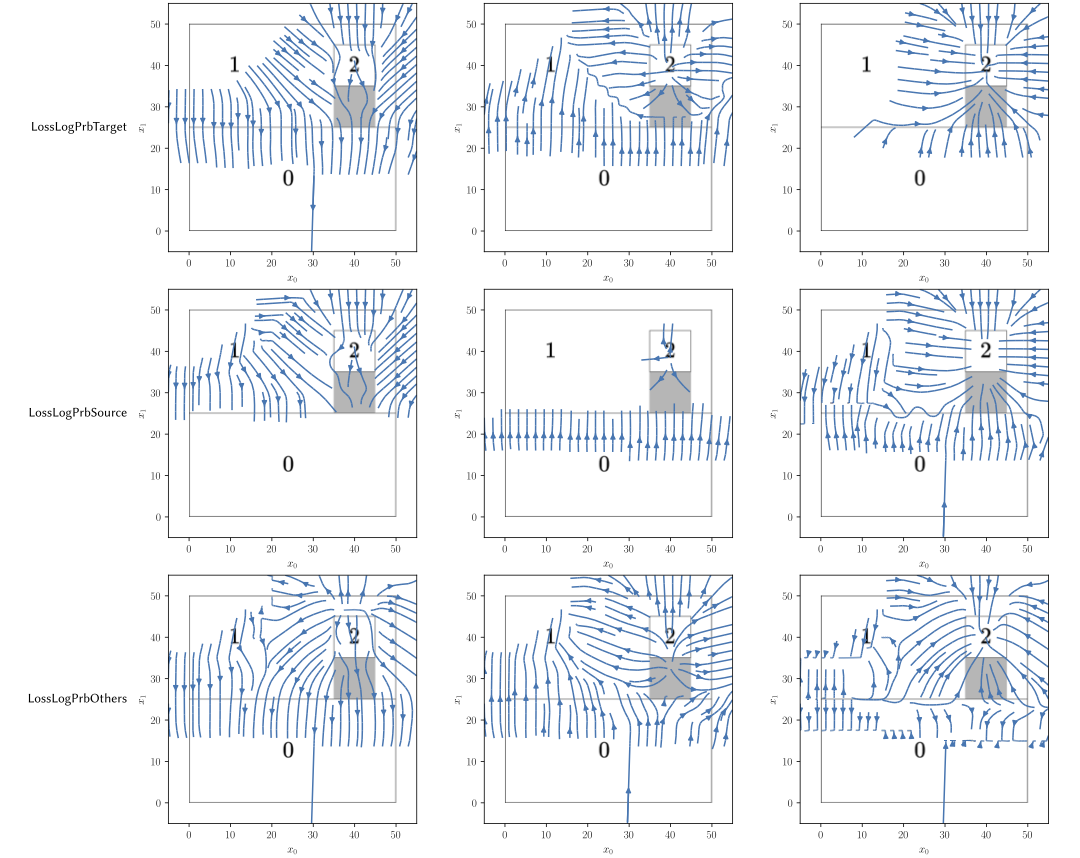
\includegraphics[width=\textwidth]{./05_cf_losses/Appendix/x_gradients_logprb.png}
        \caption{Log-probability-based losses with $\lambda=1$.}
    \end{subfigure}
    \begin{subfigure}[b]{\textwidth}
        \centering
        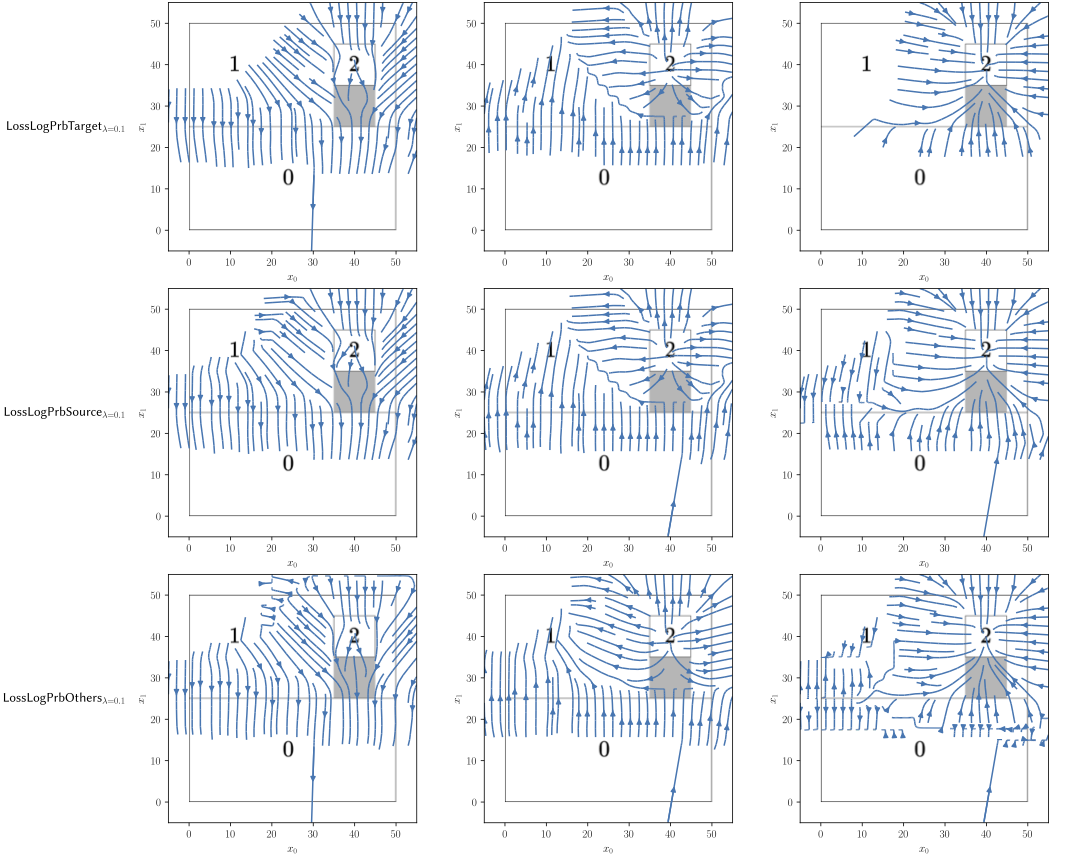
\includegraphics[width=\textwidth]{./05_cf_losses/Appendix/x_gradients_logprb01.png}
        \caption{Log-probability-based losses with $\lambda=0.1$.}
    \end{subfigure}
\end{figure}
\begin{figure}\ContinuedFloat
    \begin{subfigure}[b]{\textwidth}
        \centering
        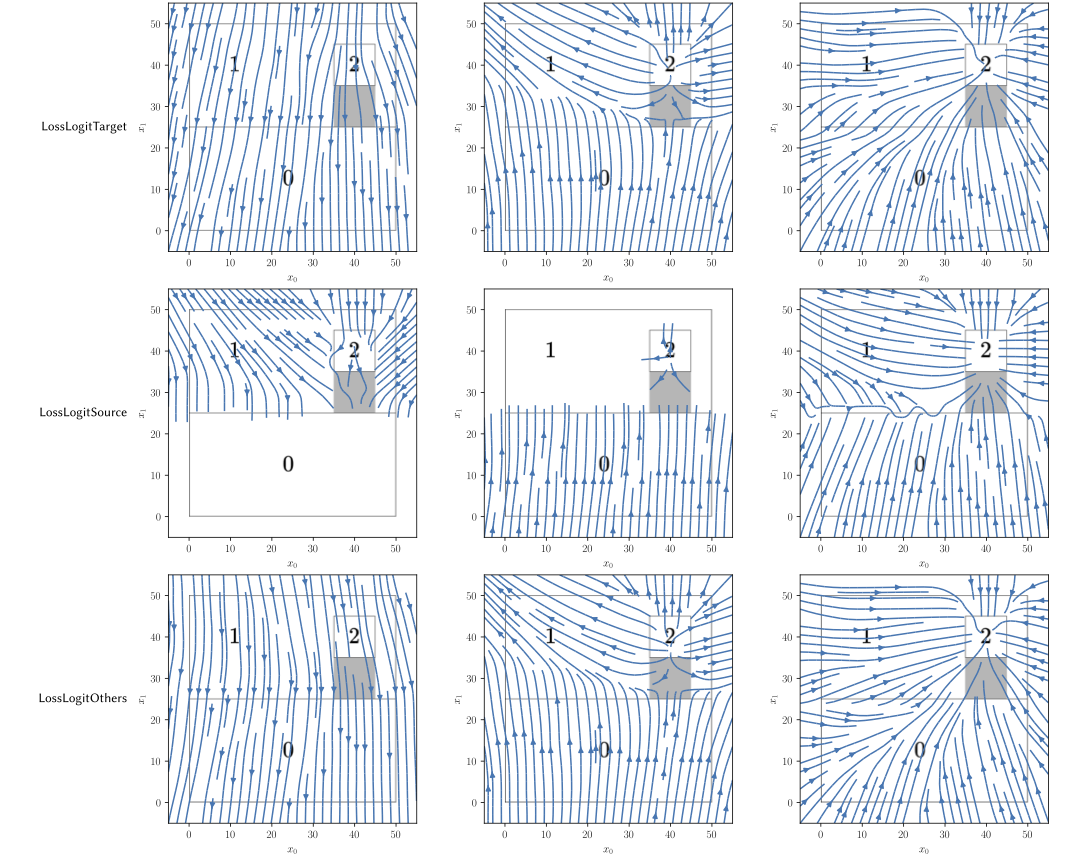
\includegraphics[width=\textwidth]{./05_cf_losses/Appendix/x_gradients_logit.png}
        \caption{Logit-based losses with $\lambda=1$.}
    \end{subfigure}
    \begin{subfigure}[b]{\textwidth}
        \centering
        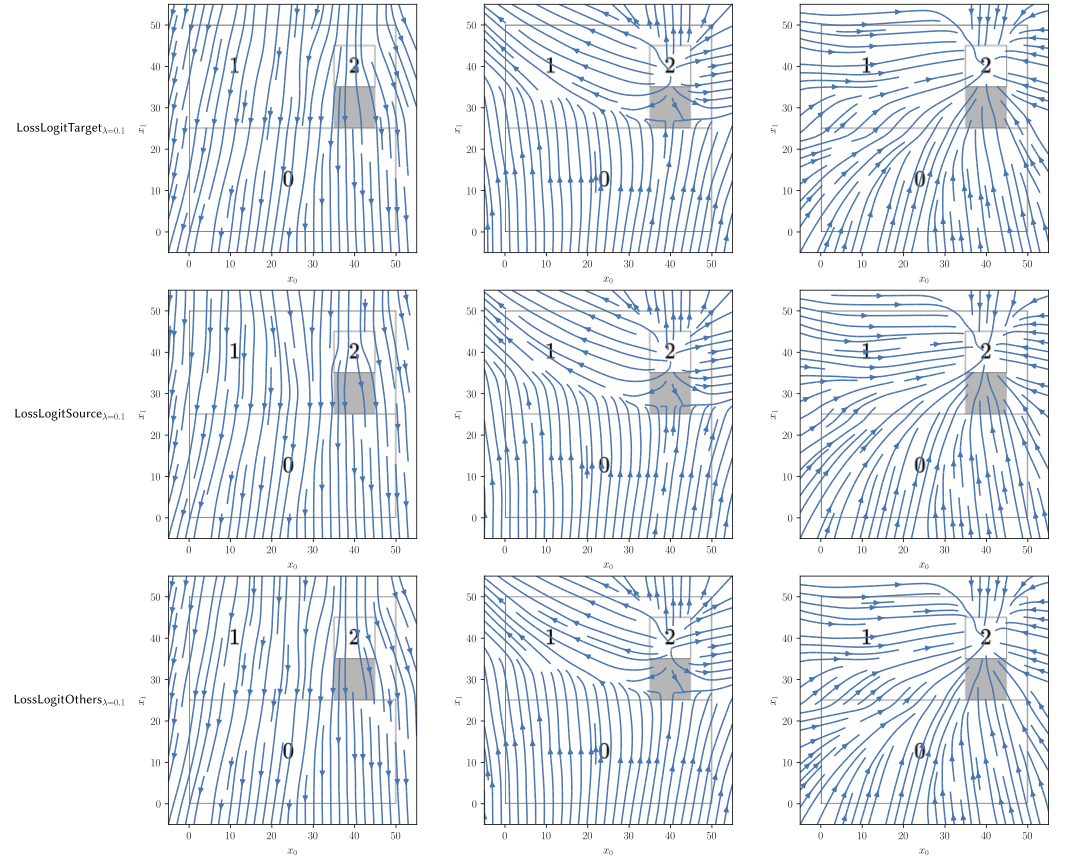
\includegraphics[width=\textwidth]{./05_cf_losses/Appendix/x_gradients_logit01.png}
        \caption{Logit-based losses with $\lambda=0.1$.}
    \end{subfigure}

    \caption{Gradients of validity losses on \CakeOnSea. The column indicates the target class.}
\end{figure}

\end{document}